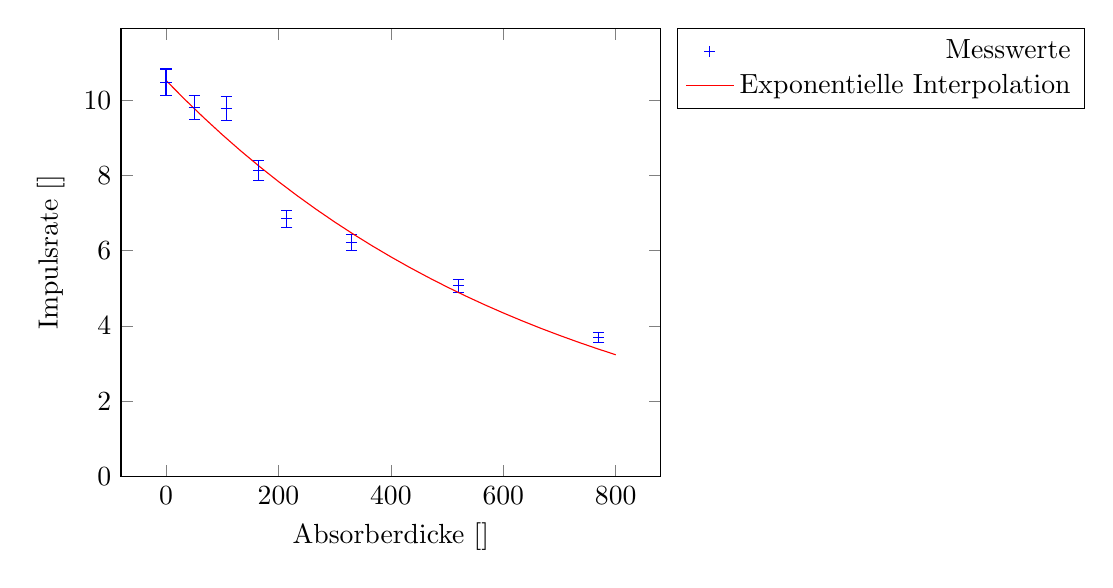
\begin{tikzpicture}
\begin{axis} [
%enlargelimits=.15,
%ybar,
%symbolic x coords={excellent, good, neutral},
%xtick = data,
error bars/y dir = both,
error bars/y explicit,
%only marks,
ymin = 0,
%ymode=log,
xlabel={Absorberdicke [\si{\micro\meter}]},
ylabel={Impulsrate [\si{\per\second}]},
legend style = {legend pos = outer north east, cells={anchor=east}}
]
\addplot+ [mark = +, only marks] table[x = x, y= y, y error = yerror]  {
x	y	yerror
0	10.4791248606	0.3480304704
50	9.8030160595	0.3249560292
107	9.7847567288	0.3231269543
165	8.1339108641	0.2695473226
215	6.847142989	0.228052825
330	6.211994003	0.206946066
520	5.0722567288	0.171892932
770	3.6943667742	0.1295697446
};
\addlegendentry{Messwerte};
\addplot+[no marks, domain=0:800] {10.52378637*exp(-1474.24606886e-6*x)};
\addlegendentry{Exponentielle Interpolation};
\end{axis}
\end{tikzpicture}